\begin{prob}[2]\textbf{Newton's Method for Unconstrained Problems:}
\end{prob}
Replicate Fig. 9.20 for the objective funciton in equation(9.20) in the textbook. Please include the
  expression for the gradient and the Hessian in your report. Also, add a few other initial starting points.

OBJECTIVE FUNCTION:
\[
\mbox{\textit{minimize }} f(x) = e^{x_{1} + 3 x_{2} - 0.1} + e^{x_{1} - 3x_{2} - 0.1} + e^{-x_{1} - 0.1}
\]

GRADIENT OF OBJECTIVE FUNCTION
\[
\nabla f(x_{1}, x_{2}) = \begin{bmatrix}
\dfrac{\partial f(x_{1}, x_{2})}{\partial x_{1}}\\
\dfrac{\partial f(x_{1}, x_{2})}{\partial x_{2}}
\end{bmatrix}
\]
where:
\begin{eqnarray*}
\dfrac{\partial f(x_{1}, x_{2})}{\partial x_{1}} &= e^{x_{1} + 3 x_{2} - 0.1} + e^{x_{1} - 3x_{2} - 0.1} - e^{-x_{1} - 0.1}\\
\dfrac{\partial f(x_{1}, x_{2})}{\partial x_{2}} &= 3 e^{x_{1} + 3 x_{2} - 0.1} - 3e^{x_{1} - 3x_{2} - 0.1}
\end{eqnarray*}
HESSIAN OF OBJECTIVE FUNCTION
\[
\nabla f(x_{1}, x_{2}) = \begin{bmatrix}
\dfrac{\partial^{2} f(x_{1}, x_{2})}{\partial x_{1}^{2}} & \dfrac{\partial^{2} f(x_{1}, x_{2})}{\partial x_{1} x_{2}}\\
\dfrac{\partial^{2} f(x_{1}, x_{2})}{\partial x_{2} x_{1}} & \dfrac{\partial^{2} f(x_{1}, x_{2})}{\partial x_{2}^{2}}
\end{bmatrix}
\]
where:
\begin{eqnarray*}
\dfrac{\partial^{2} f(x_{1}, x_{2})}{\partial x_{1}^{2}} =& e^{x_{1} + 3 x_{2} - 0.1} + e^{x_{1} - 3x_{2} - 0.1} - e^{-x_{1} - 0.1}\\
\dfrac{\partial^{2} f(x_{1}, x_{2})}{\partial x_{1} x_{2}} =& 3 e^{x_{1} + 3 x_{2} - 0.1} - 3e^{x_{1} - 3x_{2} - 0.1}\\
\dfrac{\partial^{2} f(x_{1}, x_{2})}{\partial x_{2} x_{1}} =& 3 e^{x_{1} + 3 x_{2} - 0.1} - 3e^{x_{1} - 3x_{2} - 0.1}\\
\dfrac{\partial^{2} f(x_{1}, x_{2})}{\partial x_{2}^{2}} =& 9 e^{x_{1} + 3 x_{2} - 0.1} + 9e^{x_{1} - 3x_{2} - 0.1}
\end{eqnarray*}
  \begin{figure}[H]
  \centering
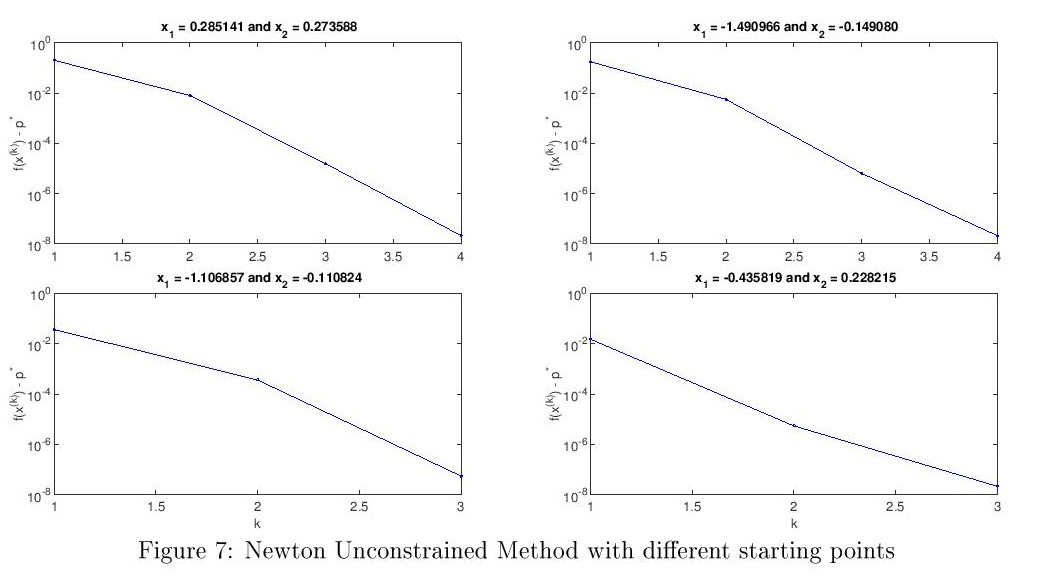
\includegraphics[width=\textwidth]{source/prob2/fig1}
%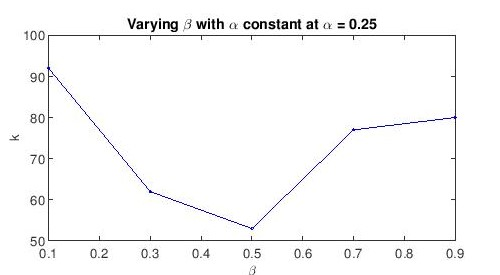
\includegraphics[width=5cm]{source/prob1/fig4}
\caption{Newton Unconstrained Method with different starting points}
\end{figure}
